\documentclass[11pt]{scrartcl}
\usepackage{amsmath}
\usepackage{amssymb}
\usepackage{epstopdf}
\usepackage{graphicx}
\usepackage{hyperref}
\usepackage[utf8]{inputenc}
\usepackage{units}
\usepackage{verbatim}

\graphicspath{{./}{../plots}}

\title{VDVC Survey}
\author{Patrik Schönfeldt}
\date{\today}

\begin{document}
\maketitle

\section{Beschreibung der Stichprobe}
\subsection{Altersstruktur}

\begin{figure}[htbp]
   \centering
   \includegraphics{2013/alter.eps} % requires the graphicx package
   \caption{Altersstruktur 2013}
   \label{fig:2013-alter}
\end{figure}

\begin{figure}[htbp]
   \centering
   \includegraphics{2014/alter} % requires the graphicx package
   \caption{Altersstruktur 2014}
   \label{fig:2014-alter}
\end{figure}


\subsection{Geschlechter}

\begin{figure}[htbp]
   \centering
   \includegraphics{2013/geschlecht} % requires the graphicx package
   \caption{Geschlechter 2013}
   \label{fig:2013-geschlecht}
\end{figure}

\begin{figure}[htbp]
   \centering
   \includegraphics{2014/geschlecht} % requires the graphicx package
   \caption{Geschlechter 2014}
   \label{fig:2014-geschlecht}
\end{figure}

\clearpage
\bibliography{VDVC-Survey}{}
\bibliographystyle{alpha}

\end{document}
